\documentclass[aspectratio=169,xcolor=pdftex,dvipsnames,table]{beamer}
\usepackage[utf8]{inputenc}
\usepackage[T1]{fontenc}
\usepackage{lmodern}
\usepackage{amsmath,amssymb,amsfonts}
\usepackage{graphicx}
\usepackage{tabularx}
\usepackage{booktabs}
\usepackage{tikz}
\usepackage{hyperref}
\usepackage{ragged2e}
\usepackage{algorithm}
\usepackage{algpseudocode}
\usepackage{float}
\usetikzlibrary{shapes.geometric, arrows, positioning}

\usetheme{Madrid}
\usecolortheme{default}
\setbeamertemplate{navigation symbols}{}
\setbeamertemplate{footline}[frame number]
\setbeamertemplate{bibliography item}[text]

\title[VQE untuk Prediksi Rezim Pasar]{Prediktibilitas Rezim Pasar dengan Algoritma Hibrida Quantum-Classical}
\date{\today}

\begin{document}

\begin{frame}
  \titlepage
\end{frame}

\begin{frame}{Agenda Presentasi}
  \tableofcontents
\end{frame}

\section{Fase 1: Representasi Matriks Kondisi Pasar}
\begin{frame}{1. Representasi Matriks Kondisi Pasar (Game Theory)}
  \begin{itemize}
    \item Pemanfaatan rekam jejak harga saham historikal yang kompetitif untuk mengkonstruksi \textbf{Matriks Payoff} berbasis Game Theory.
    \item \textbf{Fungsi Game Theory}: Berperan krusial dalam mendeteksi \textit{feedback loop} pergerakan antar aset untuk menentukan \textbf{parameter kuantum} pada Ising Hamiltonian ($\hat{H}$):
    \begin{itemize}
        \item \textbf{Bias ($h_i$)}: Dipetakan dari ekspektasi tren profitabilitas masing-masing aset indiviudal (\textit{Bullish/Bearish}).
        \item \textbf{Interaksi ($J_{ij}$)}: Diekstrak dari korelasi interaksi risiko simultan antar pasangan aset dominan dalam iklim \textit{Zero-Sum}.
    \end{itemize}
    \item \textbf{Tujuan Integrasi}: Memastikan mekanisme komputasi algoritma VQE di-\textit{feed} secara dinamis mengikuti fluktuasi pergerakan riil dari data harga historis saham di ekosistem \textit{market}.
  \end{itemize}
\end{frame}

\section{Fase 2: Transformasi ke Ising Hamiltonian}
\begin{frame}{2A. Konstruksi Objektif Markowitz \& QUBO}
  \begin{block}{Model Markowitz (Minimalisasi Risiko)}
    Tujuan optimasi portofolio dengan pembobotan aset biner $x_i \in \{0, 1\}$:
    $$ \min_x \quad w \sum_{i,j} \sigma_{ij} x_i x_j - (1-w) \sum_i \mu_i x_i $$
  \end{block}
  \vspace{0.1cm}
  Keterangan:\par
  $\sigma_{ij}$: Matriks kovariansi (korelasi risiko), \quad $\mu_i$: Ekspektasi return, \quad $w$: Toleransi risiko.
  \vspace{0.1cm}
  \begin{figure}
      \centering
      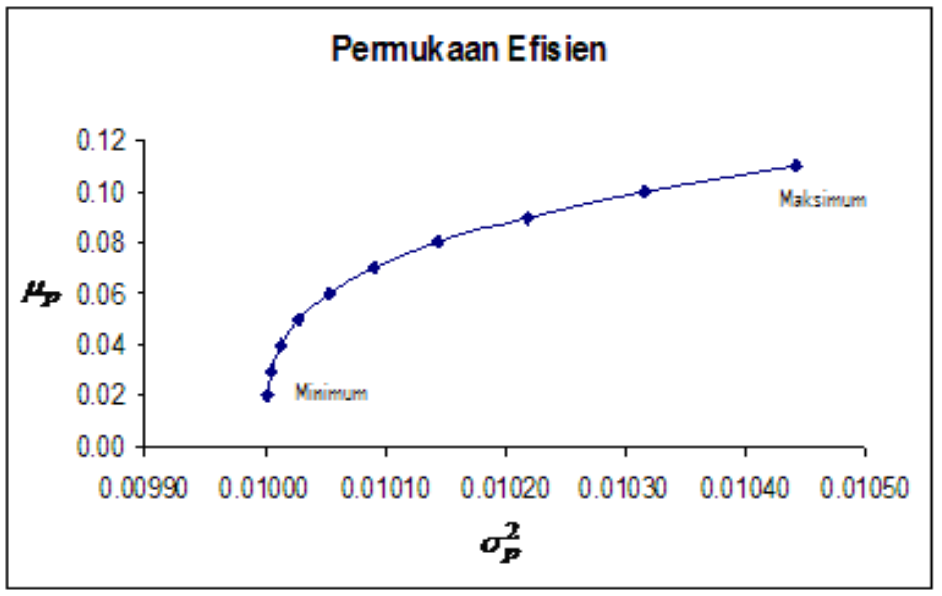
\includegraphics[height=2.5cm]{Efficient_frontier.png}
      \caption{Investasi Model Markowitz \cite{abdul_hali_markowitz_2020}}
  \end{figure}
  \vspace{0.1cm}
  \begin{alertblock}{Penalty Constraint (QUBO)}
  Transformasi batasan jumlah portofolio ($\Sigma x_i = B$) dengan skalar penalti $P$:
  $$ C(x) = w x^T \Sigma x - (1-w) \mu^T x + P \left( \sum x_i - B \right)^2 $$
  \end{alertblock}
\end{frame}

\begin{frame}{2B. Transformasi Linear ke Ising Hamiltonian ($\hat{H}$)}
  Variabel keputusan investasi klasik di-\textit{mapping} ke komputasi kuantum ke unit spin / nilai \textit{eigenvalue} operator Pauli-Z ($\hat{Z}_i \in \{+1, -1\}$):
  $$ x_i = \frac{1 - \hat{Z}_i}{2} $$
  
  \vspace{0.3cm}
  Substitusi ini mengakibatkan restrukturisasi model ekonomi makro menjadi persamaan fisika \textbf{Ising Hamiltonian}:
  $$ \hat{H} = \sum_{i} h_i \hat{Z}_i + \sum_{i<j} J_{ij} \hat{Z}_i \hat{Z}_j + \text{konstanta} $$
  
  \begin{itemize}
      \item $h_i$ (bias): Tersintesis dari probabilitas sentimen ekspektasi return.
      \item $J_{ij}$ (kopling termodinamika): Kekuatan korelasi risiko (\textit{Covariance}) antar saham.
  \end{itemize}
\end{frame}

\section{Fase 3: Implementasi VQE, Ansatz, \& Klasikal Optimisasi}
\begin{frame}{3A. Prinsip Variasional Schrodinger (VQE)}
    Karena permasalahan Hamiltonian QUBO merupakan \textit{NP-Hard}, optimisasi menggunakan komputasi hybrid \textbf{Variational Quantum Eigensolver (VQE)}.
    
    \begin{block}{Fungsi Objektif (Hukum Ekspektasi Energi)}
    Fungsi gelombang percobaan termodinamika ($|\psi(\theta)\rangle$) dipostulatkan selalu memberikan landasan atas (batas energi) bagi \textit{Ground State} aktual ($\min E_0$):
    $$ E(\theta) = \langle \psi(\theta) | \hat{H} | \psi(\theta) \rangle \geq E_0 $$
    $$ \min_{\theta} E(\theta) = \min_{\theta} \langle \psi(\theta) | \hat{H} | \psi(\theta) \rangle $$
    \end{block}
    
    Pencarian matriks konfigurasi spin dengan energi terendah ($\min E(\theta)$) setara dengan \textbf{Portfolio \& Rezim Pasar Finansial yang paling Optimal.}
\end{frame}

\begin{frame}{Ilustrasi: Sirkuit Kuantum Parameterisasi}
    \begin{figure}
        \centering
        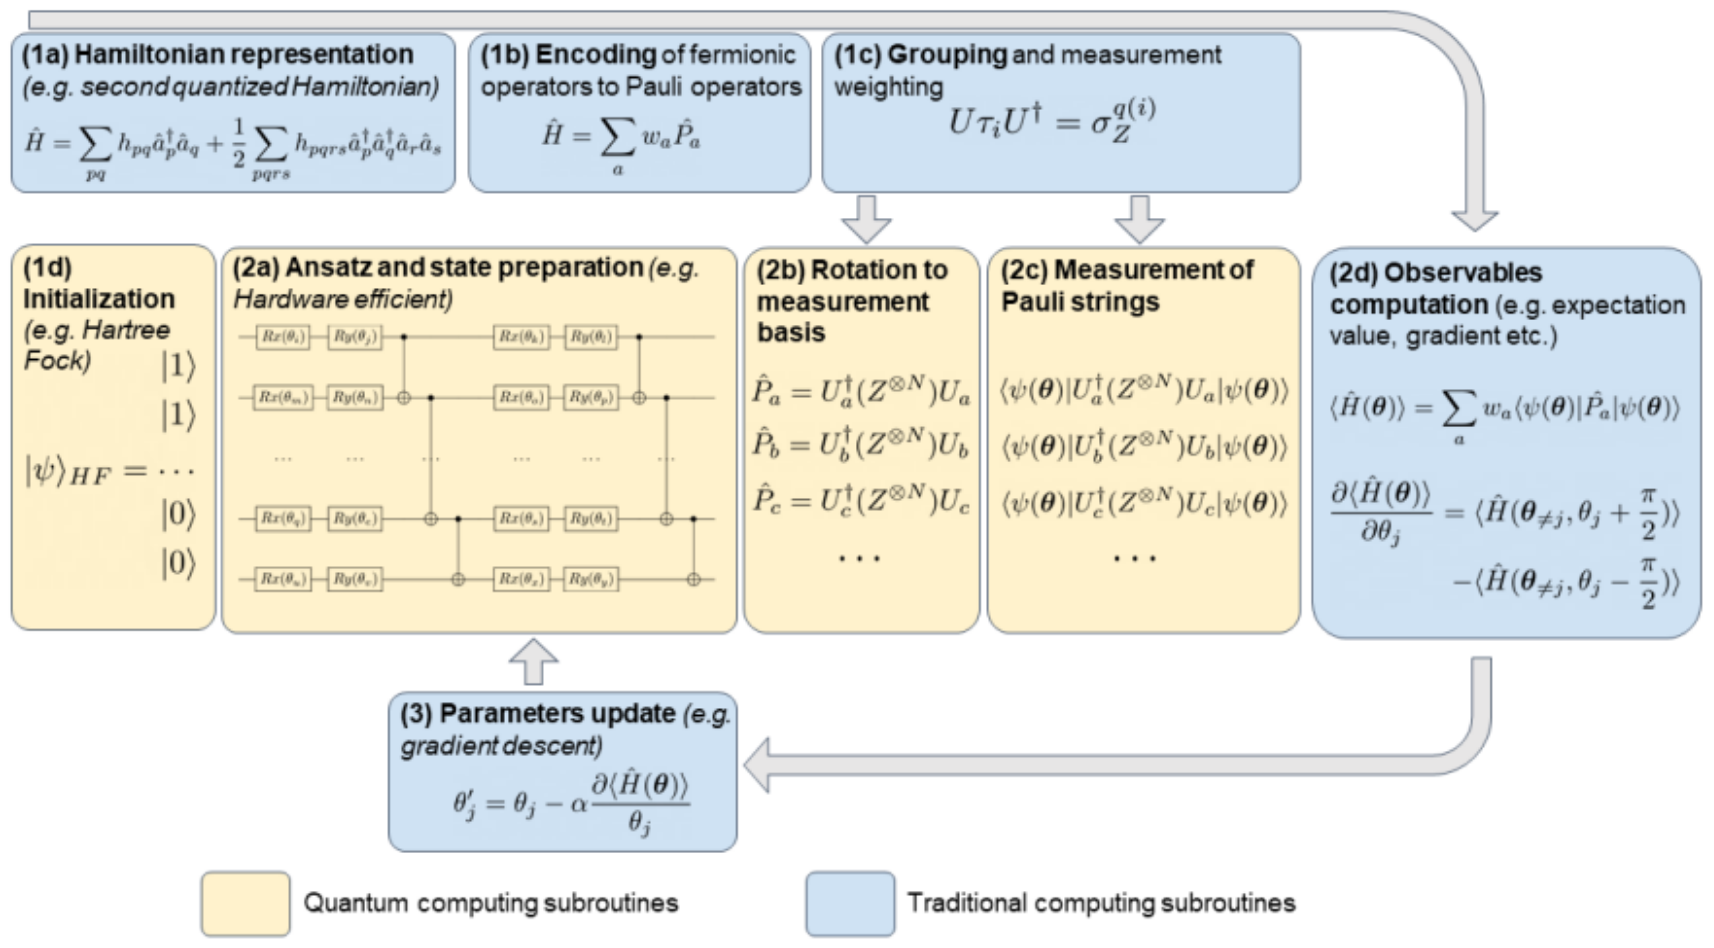
\includegraphics[height=6cm]{Quantum_gates.png}
        \caption{Sirkuit Kuantum Parameterisasi \cite{dixit_variational_2025}}
    \end{figure}
\end{frame}

\begin{frame}{Skema Hibrida VQE}
    Pencarian matriks konfigurasi spin dengan energi terendah ($\min E(\theta)$) setara dengan \textbf{Portfolio \& Rezim Pasar Finansial yang paling Optimal.}
    
    \begin{figure}
        \centering
        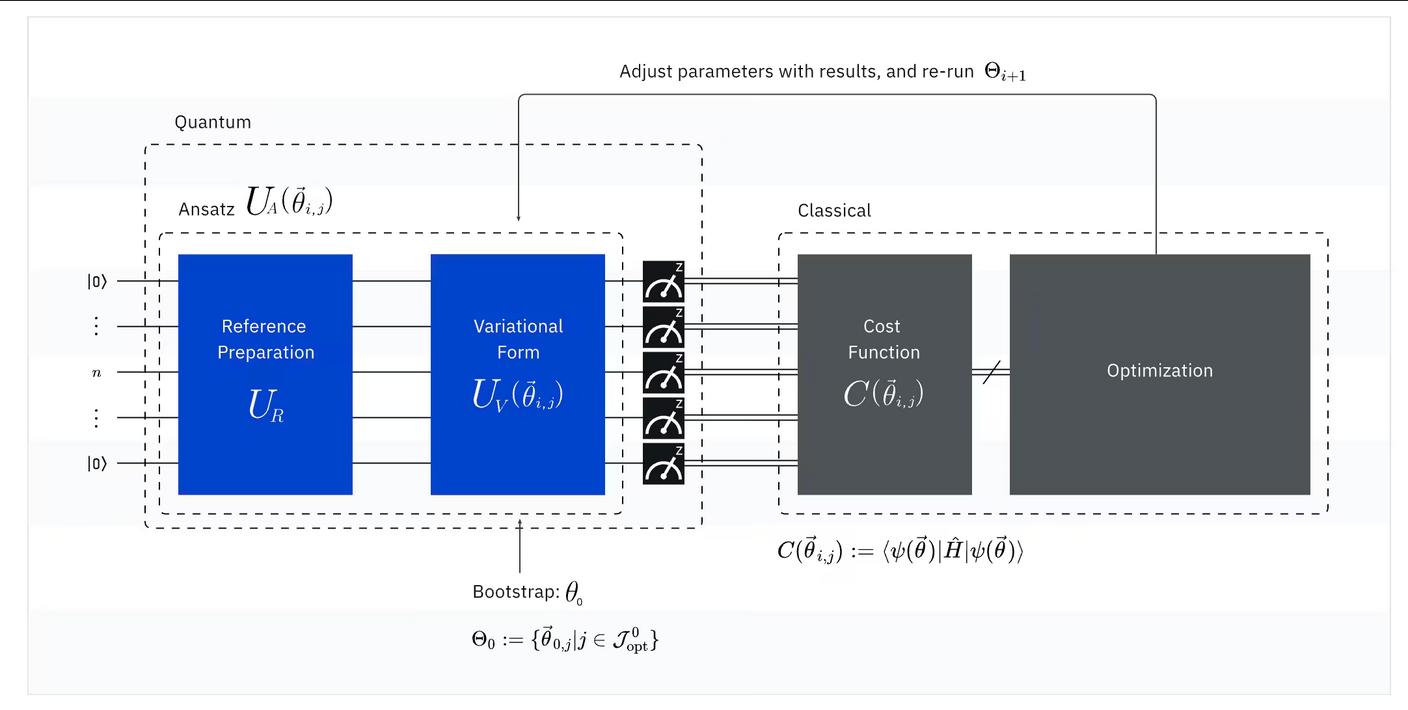
\includegraphics[height=4cm]{VQE_scheme.png}
        \caption{Skema Variational Quantum Eigensolver \footnote{\url{https://quantum.cloud.ibm.com/learning/en/modules/computer-science/vqe\#introduction}}}
    \end{figure}
\end{frame}

\begin{frame}{3B. Eksplorasi: Hardware-Efficient Ansatz (HEA)}
    Sirkuit pengevaluasi $|\psi(\theta)\rangle = \hat{U}_{ent}(\tau) |\Phi(\epsilon)\rangle$ dibangun memprioritaskan gerbang kuantum dasar tanpa abstraksi fermionik masif (*Hardware-Efficient*):
    \vspace{0.2cm}
    \begin{itemize}
        \item \textbf{Mean-Field State ($|\Phi\rangle$)}: 
        Proyeksi individual probabilitas \textit{Bullish/Bearish} dengan parameter Euler (seperti $R_y$, $R_z$).
        \item \textbf{Entanglement Blocks ($\hat{U}_{ent}$)}: Susunan persilangan \textit{exchange gates} (\textit{CNOT/CZ}) yang mereplikasi korelasional padat topologi risiko Hamiltonian ($J_{ij}$).
    \end{itemize}
    \vspace{0.2cm}
    \textbf{Keunggulan HEA}:
    Kedalaman sirkuit iteratif sangat linier dan minimum, menekan anomali di \textit{chips} kuantum \textit{Noisy Intermediate-Scale Quantum} (NISQ).
    
    \vspace{-0.2cm}
    \begin{figure}
        \centering
        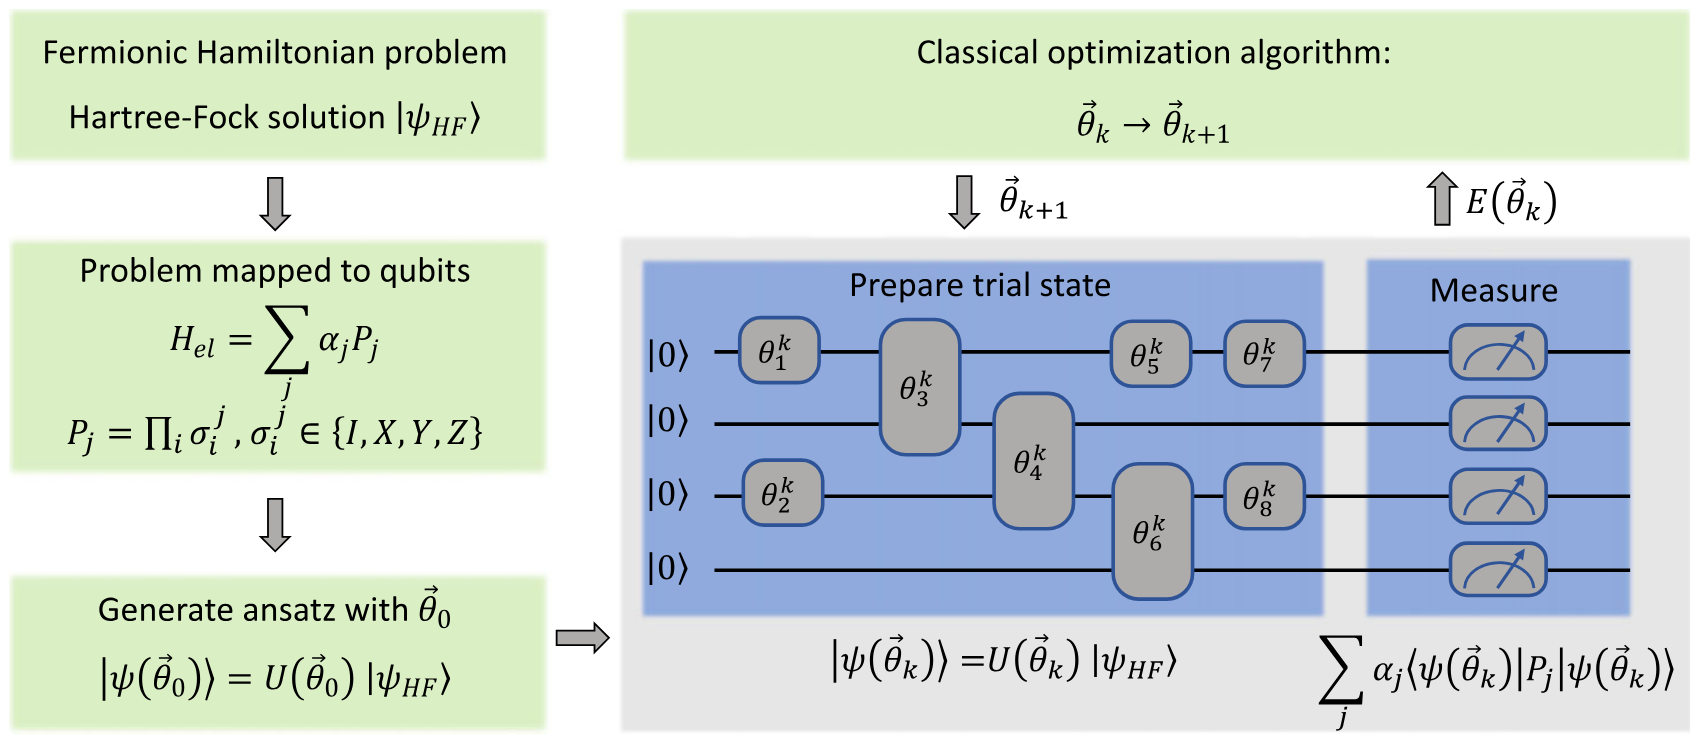
\includegraphics[height=2.5cm]{VQE_Materials_Theory.png}
        \caption{Topologi Hardware-Efficient Ansatz \cite{fedorov_vqe_2022}}
    \end{figure}
\end{frame}

\begin{frame}{3C. Optimisasi Klasik (Pendekatan Gradient Descent)}
    \begin{itemize}
        \item Fungsi biaya $E(\theta)$ diminimalkan menggunakan metode \textbf{Gradient Descent} kuantum:
        $$ \theta_{k+1} = \theta_k - \eta \nabla E(\theta_k) $$
        \item \textbf{Parameter-Shift Rule}: Gradien eksak tiap parameter $\theta_i$ dievaluasi dengan meniru prinsip turunan parsial kuantum:
        $$ \frac{\partial E}{\partial \theta_i} = \frac{E(\theta_i + \pi/2) - E(\theta_i - \pi/2)}{2} $$
        \item \textbf{Definisi Rentang Parameter Matematis}: 
        \begin{itemize}
            \item $\theta_k \in \mathbb{R}^p$: Vektor susunan parameter riil (sudut rotasi sirkuit) di iterasi $k$.
            \item $\eta \in \mathbb{R}^+$: Skalar riil positif konstan yang meregulasi ukuran fase iterasi (\textit{learning rate}).
            \item $E(\theta_k) \in \mathbb{R}$: \textit{Cost function} berupa ekspektasi energi observabel bernilai riil.
            \item $\nabla E(\theta_k) \in \mathbb{R}^p$: Vektor turunan parsial bernilai riil dari perhitungan lanskap energi.
        \end{itemize}
    \end{itemize}
\end{frame}

\begin{frame}{3D. Optimisasi Lanjutan (Pendekatan SPSA)}
    Sebagai solusi \textit{resource scaling}, digunakan \textbf{SPSA} (\textit{Simultaneous Perturbation Stochastic Approximation}) yang mengestimasi gradien fungsi biaya di sirkuit:
    $$ \hat{\theta}_{k+1} = \hat{\theta}_k - a_k \hat{g}_k(\hat{\theta}_k) $$
    $$ \hat{g}_{ki}(\hat{\theta}_k) = \frac{E(\hat{\theta}_k + c_k \Delta_k) - E(\hat{\theta}_k - c_k \Delta_k)}{2 c_k \Delta_{ki}} $$
    \begin{itemize}
        \item $\hat{g}_k(\hat{\theta}_k) \in \mathbb{R}^p$: Estimator gradien numerik multivariabel melalui perturbasi parsial (dimensi $p$).
        \item $a_k, c_k \in \mathbb{R}^+$: Skalar konstan (\textit{decaying sequences}); $a_k$ (ukuran \textit{learning step}), $c_k$ (ukuran \textit{shift/perturbation}).
        \item $\Delta_k \in \{-1, +1\}^p$: Vektor perturbasi dimensi-$p$ asimetris yang dihasilkan dari \textbf{Distribusi Rademacher} bebas (probabilitas acak non-nol dengan rata-rata 0).
        \item $\Delta_{ki}$: Entri spesifik indeks $i$ pada nilai vektor ekspektasi acak $\Delta_k$.
    \end{itemize}
\end{frame}

\section{Fase 4: Realisasi \& Interpretasi Eksekusi Portofolio}
\begin{frame}{4. Interpretasi \& Pemetaan Rezim Portofolio}
  Ketika perhitungan mencapai titik stasioner (konvergensi absolut $\Delta E \approx 0$), sirkuit ansatz dengan $\theta_{opt}$ diproyeksikan (ribuan \textit{shots measurement}).
  \vspace{0.2cm}
  
  \begin{block}{Interpretasi Nilai Probabilitas $Z$}  
  \textbf{Resolusi Bitstring Ekspektasi Maksimal: $|1100\rangle$}
  \begin{itemize}
      \item Saham A: $+1$ (Proyeksi \textit{Bullish} - Alokasi Modal Dominan)
      \item Saham B: $+1$ (Proyeksi \textit{Bullish} - Alokasi Modal Dominan)
      \item Saham C: $-1$ (Proyeksi \textit{Bearish} - Hindari / Jual)
      \item Saham D: $-1$ (Proyeksi \textit{Bearish} - Hindari / Jual)
  \end{itemize}
  \end{block}
  Rekomendasi metode \textit{Quantum Game Theory} ini menawarkan signifikansi analitik alokasi absolut dalam keseimbangan ekosistem pasar (\textit{Zero-Sum Tolerance}), memastikan ketahanan resistensi tertinggi melawan anomali pasar (\textit{trend deviation}).
\end{frame}

\begin{frame}{Pseudocode Variational Quantum Eigensolver}
  \begin{algorithm}[H]
    \caption{Variational Quantum Eigensolver (VQE)}
    \begin{algorithmic}[1]
      \Require Hamiltonian $H$, ansatz $U(\boldsymbol{\theta})$, classical optimizer $\mathcal{O}$
      \Ensure Approximate ground-state energy $E^*$
      \State Initialize parameters $\boldsymbol{\theta}$
      \Repeat
        \State Prepare trial state $|\psi(\boldsymbol{\theta})\rangle = U(\boldsymbol{\theta}) |0\rangle$
        \State Estimate energy $E(\boldsymbol{\theta}) = \langle\psi(\boldsymbol{\theta})| H |\psi(\boldsymbol{\theta})\rangle$ via repeated measurements
        \State Update parameters $\boldsymbol{\theta} \leftarrow \mathcal{O}(\boldsymbol{\theta}, \nabla_{\theta} E)$
      \Until{convergence}
      \State \textbf{return} $E^* = E(\boldsymbol{\theta})$
    \end{algorithmic}
  \end{algorithm}
  \vspace{0.1cm}
  \centering \footnotesize Sumber: \cite{dixit_variational_2025}
\end{frame}

\begin{frame}{Alur Kerja VQE Pendeteksi Prediksi Pasar}
\centering
\tikzstyle{startstop} = [rectangle, rounded corners, minimum width=2.5cm, minimum height=0.8cm,text centered, draw=black, fill=red!30]
\tikzstyle{io} = [trapezium, trapezium left angle=70, trapezium right angle=110, minimum width=2.5cm, minimum height=0.8cm, text centered, draw=black, fill=blue!20]
\tikzstyle{process} = [rectangle, minimum width=3cm, minimum height=0.8cm, text centered, draw=black, fill=orange!20, text width=4cm]
\tikzstyle{decision} = [diamond, minimum width=2.5cm, minimum height=1cm, text centered, draw=black, fill=green!20, aspect=2, text width=2.5cm]
\tikzstyle{arrow} = [thick,->,>=stealth]

\resizebox{0.9\textwidth}{!}{%
\begin{tikzpicture}[node distance=1.8cm]

% Nodes
\node (in1) [io] {Data Historis Return 4 Aset};
\node (pro1) [process, below of=in1, yshift=-0.2cm] {Representasi Kuantifikasi Matriks Kondisi Bullish/Bearish};
\node (pro2) [process, below of=pro1] {Transformasi Matriks ke Formulasi QUBO (\textbf{Penalty})};
\node (pro3) [process, below of=pro2] {Pembentukan Observable (Ising Hamiltonian $\hat{H}$)};
\node (pro4) [process, below of=pro3] {Inisiasi VQE Parameter \& \textbf{HEA Circuit}};

\node (pro5) [process, right of=pro4, xshift=5.5cm, fill=purple!20] {Eksekusi Observasi Energi ($E_{\text{approx}}$) di QPU};
\node (dec1) [decision, above of=pro5, yshift=1cm] {Apakah $\Delta E \approx 0$?};
\node (pro6) [process, above of=dec1, yshift=1.5cm, fill=cyan!20] {Aproksimasi Derivatif Stokastik (SPSA Optimizer)};

\node (out1) [io, right of=dec1, xshift=4.5cm, align=center] {Parameter Optimal $\theta_{opt}$ \\ (Ground State)};
\node (pro7) [process, below of=out1, yshift=-0.5cm] {Ekstraksi Distribusi \\ Shots ($|1100\rangle$)};
\node (stop) [startstop, below of=pro7, yshift=-0.5cm] {Keputusan Rezim Pasar};

% Arrows
\draw [arrow] (in1) -- (pro1);
\draw [arrow] (pro1) -- (pro2);
\draw [arrow] (pro2) -- (pro3);
\draw [arrow] (pro3) -- (pro4);
\draw [arrow] (pro4) -- (pro5);
\draw [arrow] (pro5) -- (dec1);

\draw [arrow] (dec1) -- node[anchor=east] {Tidak} (pro6);
\draw [arrow] (pro6.west) -- ++(-1.5,0) |- node[anchor=north] {Update $\theta_{k+1}$} (pro5.west);
\draw [arrow] (dec1) -- node[anchor=north] {Ya} (out1);

\draw [arrow] (out1) -- (pro7);
\draw [arrow] (pro7) -- (stop);

\end{tikzpicture}
}
\end{frame}

\begin{frame}[allowframebreaks]{Daftar Pustaka}
    \begin{thebibliography}{10}
        \bibitem{abdul_hali_markowitz_2020}
        N. Abdul Hali and A. Yuliati, ``Markowitz Model Investment Portfolio Optimization: a Review Theory,'' \textit{International Journal of Research in Community Services}, vol. 1, no. 3, pp. 14--18, Oct. 2020, doi: \url{https://doi.org/10.46336/ijrcs.v1i3.104}.
        
        \bibitem{fedorov_vqe_2022}
        D. A. Fedorov, B. Peng, N. Govind, and Y. Alexeev, ``VQE method: a short survey and recent developments,'' \textit{Materials Theory}, vol. 6, no. 1, p. 2, Jan. 2022, doi: \url{https://doi.org/10.1186/s41313-021-00032-6}.
        
        \bibitem{dixit_variational_2025}
        A. Dixit and A. Kumari, ``Variational Principle 2.0: The Variational Quantum Eigensolver,'' Nov. 2025.
    \end{thebibliography}
\end{frame}

\end{document}
